\chapter{Approach and Implementation}
\label{chapter:Approach}

\begin{itemize}
\item What's your general approach to answer your questions?
\item What were different design decisions/options? Which one did you chose?
What are the pros and cons?
\item What did you implement? (including a description of your PoC)
\end{itemize}

This is most likely your main part! Probably 10-25 pages. Can also be split up
into two or more chapters depending on your work. Probably, it makes sense to
break down the title of your thesis into multiple components and make a section
for each of them.

It often makes sense to start with a description of the steps of your program
with a nice (yet often similar) visual representation as shown in Figure
\ref{fig:tool_overview}. If you're not familiar with \texttt{tikz} and so on, I
recommend using draw.io\footnote{\url{https://app.diagrams.net/}} and export the
figure as pdf. (Hint: you can also track the .drawio file in git --- it's a
simple xml format).

\begin{figure}[ht]
\centering
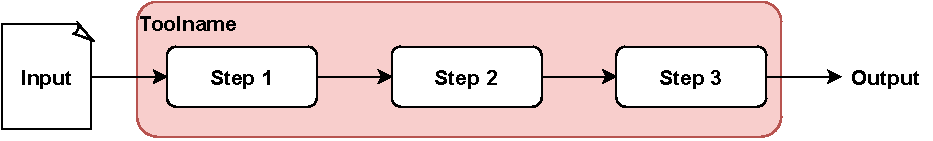
\includegraphics[width=0.8\textwidth]{figures/generic_figure.pdf}
\caption{Workflow of my amazing tool}
\label{fig:tool_overview}
\end{figure}


Similarly, create tables and please, always explain and reference the tables,
figures, listings in the text with a reference. Examples are Table
\ref{tab:example_tab} summarizing the medals won during the Olympics 2021 for
the top 3 nations or Listing \ref{lst:fac} calculating the factorial of the
input.

\begin{table}[ht]
\centering
\caption{Olympics 2021: Medals of top 3 nations.}
\label{tab:example_tab}
\begin{tabular}{| l | c | c | c |}\hline
& \textbf{Gold} & \textbf{Silver} & \textbf{Bronze}\\\hline
\textbf{USA} & 39 & 41 & 33 \\\hline
\textbf{China} & 38 & 32 & 18 \\\hline
\textbf{Japan} & 27 & 14 & 17 \\\hline
\end{tabular}
\end{table}

\begin{lstlisting}[language=python,caption={Function computing the factorial},label={lst:fac}]
def frac(n):
    if n == 1:
        return 1
    return n * frac(n-1)
\end{lstlisting}
